
%% bare_jrnl.tex
%% V1.4
%% 2012/12/27
%% by Michael Shell
%% see http://www.michaelshell.org/
%% for current contact information.
%%
%% This is a skeleton file demonstrating the use of IEEEtran.cls
%% (requires IEEEtran.cls version 1.8 or later) with an IEEE journal paper.
%%
%% Support sites:
%% http://www.michaelshell.org/tex/ieeetran/
%% http://www.ctan.org/tex-archive/macros/latex/contrib/IEEEtran/
%% and
%% http://www.ieee.org/



% *** Authors should verify (and, if needed, correct) their LaTeX system  ***
% *** with the testflow diagnostic prior to trusting their LaTeX platform ***
% *** with production work. IEEE's font choices can trigger bugs that do  ***
% *** not appear when using other class files.                            ***
% The testflow support page is at:
% http://www.michaelshell.org/tex/testflow/


%%*************************************************************************
%% Legal Notice:
%% This code is offered as-is without any warranty either expressed or
%% implied; without even the implied warranty of MERCHANTABILITY or
%% FITNESS FOR A PARTICULAR PURPOSE! 
%% User assumes all risk.
%% In no event shall IEEE or any contributor to this code be liable for
%% any damages or losses, including, but not limited to, incidental,
%% consequential, or any other damages, resulting from the use or misuse
%% of any information contained here.
%%
%% All comments are the opinions of their respective authors and are not
%% necessarily endorsed by the IEEE.
%%
%% This work is distributed under the LaTeX Project Public License (LPPL)
%% ( http://www.latex-project.org/ ) version 1.3, and may be freely used,
%% distributed and modified. A copy of the LPPL, version 1.3, is included
%% in the base LaTeX documentation of all distributions of LaTeX released
%% 2003/12/01 or later.
%% Retain all contribution notices and credits.
%% ** Modified files should be clearly indicated as such, including  **
%% ** renaming them and changing author support contact information. **
%%
%% File list of work: IEEEtran.cls, IEEEtran_HOWTO.pdf, bare_adv.tex,
%%                    bare_conf.tex, bare_jrnl.tex, bare_jrnl_compsoc.tex,
%%                    bare_jrnl_transmag.tex
%%*************************************************************************

% Note that the a4paper option is mainly intended so that authors in
% countries using A4 can easily print to A4 and see how their papers will
% look in print - the typesetting of the document will not typically be
% affected with changes in paper size (but the bottom and side margins will).
% Use the testflow package mentioned above to verify correct handling of
% both paper sizes by the user's LaTeX system.
%
% Also note that the "draftcls" or "draftclsnofoot", not "draft", option
% should be used if it is desired that the figures are to be displayed in
% draft mode.
%
\documentclass[journal,onecolumn]{IEEEtran}
%
% If IEEEtran.cls has not been installed into the LaTeX system files,
% manually specify the path to it like:
% \documentclass[journal]{../sty/IEEEtran}





% Some very useful LaTeX packages include:
% (uncomment the ones you want to load)


% *** MISC UTILITY PACKAGES ***
%
%\usepackage{ifpdf}
% Heiko Oberdiek's ifpdf.sty is very useful if you need conditional
% compilation based on whether the output is pdf or dvi.
% usage:
% \ifpdf
%   % pdf code
% \else
%   % dvi code
% \fi
% The latest version of ifpdf.sty can be obtained from:
% http://www.ctan.org/tex-archive/macros/latex/contrib/oberdiek/
% Also, note that IEEEtran.cls V1.7 and later provides a builtin
% \ifCLASSINFOpdf conditional that works the same way.
% When switching from latex to pdflatex and vice-versa, the compiler may
% have to be run twice to clear warning/error messages.

% \usepackage[
% backend=biber,
% ]{biblatex}
% \addbibresource{references.bib}



\usepackage{blindtext}
\usepackage{caption}
\usepackage{subcaption}
\usepackage{graphicx}
\usepackage{soul}
\usepackage{color}


\newenvironment{Figure}
  {\par\medskip\noindent\minipage{\linewidth}}
  {\endminipage\par\medskip}


% *** CITATION PACKAGES ***
%
\usepackage{cite}
% cite.sty was written by Donald Arseneau
% V1.6 and later of IEEEtran pre-defines the format of the cite.sty package
% \cite{} output to follow that of IEEE. Loading the cite package will
% result in citation numbers being automatically sorted and properly
% "compressed/ranged". e.g., [1], [9], [2], [7], [5], [6] without using
% cite.sty will become [1], [2], [5]--[7], [9] using cite.sty. cite.sty's
% \cite will automatically add leading space, if needed. Use cite.sty's
% noadjust option (cite.sty V3.8 and later) if you want to turn this off
% such as if a citation ever needs to be enclosed in parenthesis.
% cite.sty is already installed on most LaTeX systems. Be sure and use
% version 4.0 (2003-05-27) and later if using hyperref.sty. cite.sty does
% not currently provide for hyperlinked citations.
% The latest version can be obtained at:
% http://www.ctan.org/tex-archive/macros/latex/contrib/cite/
% The documentation is contained in the cite.sty file itself.






% *** GRAPHICS RELATED PACKAGES ***
%
\ifCLASSINFOpdf
  % \usepackage[pdftex]{graphicx}
  % declare the path(s) where your graphic files are
  % \graphicspath{{../pdf/}{../jpeg/}}
  % and their extensions so you won't have to specify these with
  % every instance of \includegraphics
  % \DeclareGraphicsExtensions{.pdf,.jpeg,.png}
\else
  % or other class option (dvipsone, dvipdf, if not using dvips). graphicx
  % will default to the driver specified in the system graphics.cfg if no
  % driver is specified.
  % \usepackage[dvips]{graphicx}
  % declare the path(s) where your graphic files are
  % \graphicspath{{../eps/}}
  % and their extensions so you won't have to specify these with
  % every instance of \includegraphics
  % \DeclareGraphicsExtensions{.eps}
\fi
% graphicx was written by David Carlisle and Sebastian Rahtz. It is
% required if you want graphics, photos, etc. graphicx.sty is already
% installed on most LaTeX systems. The latest version and documentation
% can be obtained at: 
% http://www.ctan.org/tex-archive/macros/latex/required/graphics/
% Another good source of documentation is "Using Imported Graphics in
% LaTeX2e" by Keith Reckdahl which can be found at:
% http://www.ctan.org/tex-archive/info/epslatex/
%
% latex, and pdflatex in dvi mode, support graphics in encapsulated
% postscript (.eps) format. pdflatex in pdf mode supports graphics
% in .pdf, .jpeg, .png and .mps (metapost) formats. Users should ensure
% that all non-photo figures use a vector format (.eps, .pdf, .mps) and
% not a bitmapped formats (.jpeg, .png). IEEE frowns on bitmapped formats
% which can result in "jaggedy"/blurry rendering of lines and letters as
% well as large increases in file sizes.
%
% You can find documentation about the pdfTeX application at:
% http://www.tug.org/applications/pdftex





% *** MATH PACKAGES ***
%
%\usepackage[cmex10]{amsmath}
% A popular package from the American Mathematical Society that provides
% many useful and powerful commands for dealing with mathematics. If using
% it, be sure to load this package with the cmex10 option to ensure that
% only type 1 fonts will utilized at all point sizes. Without this option,
% it is possible that some math symbols, particularly those within
% footnotes, will be rendered in bitmap form which will result in a
% document that can not be IEEE Xplore compliant!
%
% Also, note that the amsmath package sets \interdisplaylinepenalty to 10000
% thus preventing page breaks from occurring within multiline equations. Use:
%\interdisplaylinepenalty=2500
% after loading amsmath to restore such page breaks as IEEEtran.cls normally
% does. amsmath.sty is already installed on most LaTeX systems. The latest
% version and documentation can be obtained at:
% http://www.ctan.org/tex-archive/macros/latex/required/amslatex/math/





% *** SPECIALIZED LIST PACKAGES ***
%
%\usepackage{algorithmic}
% algorithmic.sty was written by Peter Williams and Rogerio Brito.
% This package provides an algorithmic environment fo describing algorithms.
% You can use the algorithmic environment in-text or within a figure
% environment to provide for a floating algorithm. Do NOT use the algorithm
% floating environment provided by algorithm.sty (by the same authors) or
% algorithm2e.sty (by Christophe Fiorio) as IEEE does not use dedicated
% algorithm float types and packages that provide these will not provide
% correct IEEE style captions. The latest version and documentation of
% algorithmic.sty can be obtained at:
% http://www.ctan.org/tex-archive/macros/latex/contrib/algorithms/
% There is also a support site at:
% http://algorithms.berlios.de/index.html
% Also of interest may be the (relatively newer and more customizable)
% algorithmicx.sty package by Szasz Janos:
% http://www.ctan.org/tex-archive/macros/latex/contrib/algorithmicx/




% *** ALIGNMENT PACKAGES ***
%
%\usepackage{array}
% Frank Mittelbach's and David Carlisle's array.sty patches and improves
% the standard LaTeX2e array and tabular environments to provide better
% appearance and additional user controls. As the default LaTeX2e table
% generation code is lacking to the point of almost being broken with
% respect to the quality of the end results, all users are strongly
% advised to use an enhanced (at the very least that provided by array.sty)
% set of table tools. array.sty is already installed on most systems. The
% latest version and documentation can be obtained at:
% http://www.ctan.org/tex-archive/macros/latex/required/tools/


% IEEEtran contains the IEEEeqnarray family of commands that can be used to
% generate multiline equations as well as matrices, tables, etc., of high
% quality.



% *** SUBFIGURE PACKAGES ***
%\ifCLASSOPTIONcompsoc
%  \usepackage[caption=false,font=normalsize,labelfont=sf,textfont=sf]{subfig}
%\else
%  \usepackage[caption=false,font=footnotesize]{subfig}
%\fi
% subfig.sty, written by Steven Douglas Cochran, is the modern replacement
% for subfigure.sty, the latter of which is no longer maintained and is
% incompatible with some LaTeX packages including fixltx2e. However,
% subfig.sty requires and automatically loads Axel Sommerfeldt's caption.sty
% which will override IEEEtran.cls' handling of captions and this will result
% in non-IEEE style figure/table captions. To prevent this problem, be sure
% and invoke subfig.sty's "caption=false" package option (available since
% subfig.sty version 1.3, 2005/06/28) as this is will preserve IEEEtran.cls
% handling of captions.
% Note that the Computer Society format requires a larger sans serif font
% than the serif footnote size font used in traditional IEEE formatting
% and thus the need to invoke different subfig.sty package options depending
% on whether compsoc mode has been enabled.
%
% The latest version and documentation of subfig.sty can be obtained at:
% http://www.ctan.org/tex-archive/macros/latex/contrib/subfig/




% *** FLOAT PACKAGES ***
%
%\usepackage{fixltx2e}
% fixltx2e, the successor to the earlier fix2col.sty, was written by
% Frank Mittelbach and David Carlisle. This package corrects a few problems
% in the LaTeX2e kernel, the most notable of which is that in current
% LaTeX2e releases, the ordering of single and double column floats is not
% guaranteed to be preserved. Thus, an unpatched LaTeX2e can allow a
% single column figure to be placed prior to an earlier double column
% figure. The latest version and documentation can be found at:
% http://www.ctan.org/tex-archive/macros/latex/base/


%\usepackage{stfloats}
% stfloats.sty was written by Sigitas Tolusis. This package gives LaTeX2e
% the ability to do double column floats at the bottom of the page as well
% as the top. (e.g., "\begin{figure*}[!b]" is not normally possible in
% LaTeX2e). It also provides a command:
%\fnbelowfloat
% to enable the placement of footnotes below bottom floats (the standard
% LaTeX2e kernel puts them above bottom floats). This is an invasive package
% which rewrites many portions of the LaTeX2e float routines. It may not work
% with other packages that modify the LaTeX2e float routines. The latest
% version and documentation can be obtained at:
% http://www.ctan.org/tex-archive/macros/latex/contrib/sttools/
% Do not use the stfloats baselinefloat ability as IEEE does not allow
% \baselineskip to stretch. Authors submitting work to the IEEE should note
% that IEEE rarely uses double column equations and that authors should try
% to avoid such use. Do not be tempted to use the cuted.sty or midfloat.sty
% packages (also by Sigitas Tolusis) as IEEE does not format its papers in
% such ways.
% Do not attempt to use stfloats with fixltx2e as they are incompatible.
% Instead, use Morten Hogholm'a dblfloatfix which combines the features
% of both fixltx2e and stfloats:
%
% \usepackage{dblfloatfix}
% The latest version can be found at:
% http://www.ctan.org/tex-archive/macros/latex/contrib/dblfloatfix/




%\ifCLASSOPTIONcaptionsoff
%  \usepackage[nomarkers]{endfloat}
% \let\MYoriglatexcaption\caption
% \renewcommand{\caption}[2][\relax]{\MYoriglatexcaption[#2]{#2}}
%\fi
% endfloat.sty was written by James Darrell McCauley, Jeff Goldberg and 
% Axel Sommerfeldt. This package may be useful when used in conjunction with 
% IEEEtran.cls'  captionsoff option. Some IEEE journals/societies require that
% submissions have lists of figures/tables at the end of the paper and that
% figures/tables without any captions are placed on a page by themselves at
% the end of the document. If needed, the draftcls IEEEtran class option or
% \CLASSINPUTbaselinestretch interface can be used to increase the line
% spacing as well. Be sure and use the nomarkers option of endfloat to
% prevent endfloat from "marking" where the figures would have been placed
% in the text. The two hack lines of code above are a slight modification of
% that suggested by in the endfloat docs (section 8.4.1) to ensure that
% the full captions always appear in the list of figures/tables - even if
% the user used the short optional argument of \caption[]{}.
% IEEE papers do not typically make use of \caption[]'s optional argument,
% so this should not be an issue. A similar trick can be used to disable
% captions of packages such as subfig.sty that lack options to turn off
% the subcaptions:
% For subfig.sty:
% \let\MYorigsubfloat\subfloat
% \renewcommand{\subfloat}[2][\relax]{\MYorigsubfloat[]{#2}}
% However, the above trick will not work if both optional arguments of
% the \subfloat command are used. Furthermore, there needs to be a
% description of each subfigure *somewhere* and endfloat does not add
% subfigure captions to its list of figures. Thus, the best approach is to
% avoid the use of subfigure captions (many IEEE journals avoid them anyway)
% and instead reference/explain all the subfigures within the main caption.
% The latest version of endfloat.sty and its documentation can obtained at:
% http://www.ctan.org/tex-archive/macros/latex/contrib/endfloat/
%
% The IEEEtran \ifCLASSOPTIONcaptionsoff conditional can also be used
% later in the document, say, to conditionally put the References on a 
% page by themselves.




% *** PDF, URL AND HYPERLINK PACKAGES ***
%
%\usepackage{url}
% url.sty was written by Donald Arseneau. It provides better support for
% handling and breaking URLs. url.sty is already installed on most LaTeX
% systems. The latest version and documentation can be obtained at:
% http://www.ctan.org/tex-archive/macros/latex/contrib/url/
% Basically, \url{my_url_here}.




% *** Do not adjust lengths that control margins, column widths, etc. ***
% *** Do not use packages that alter fonts (such as pslatex).         ***
% There should be no need to do such things with IEEEtran.cls V1.6 and later.
% (Unless specifically asked to do so by the journal or conference you plan
% to submit to, of course. )


% correct bad hyphenation here
\hyphenation{op-tical net-works semi-conduc-tor}


\begin{document}
%
% paper title
% can use linebreaks \\ within to get better formatting as desired
% Do not put math or special symbols in the title.
\title{ StyleArm: a style-transferring robot arm.}
%
%
% author names and IEEE memberships
% note positions of commas and nonbreaking spaces ( ~ ) LaTeX will not break
% a structure at a ~ so this keeps an author's name from being broken across
% two lines.
% use \thanks{} to gain access to the first footnote area
% a separate \thanks must be used for each paragraph as LaTeX2e's \thanks
% was not built to handle multiple paragraphs
%

\author{ Vernon Stanley Albayeros Duarte% <-this % stops a space
\thanks{Author: Vernon Stanley Albayeros Duarte, stanley.albayeros@gmail.com}% <-this % stops a space
\thanks{Advisor: Fernando Vilariño, Computer Vision Centre,  Universitat Autònoma de Barcelona }% <-this % stops a space
\thanks{Thesis dissertation submitted: September 2021}}

% note the % following the last \IEEEmembership and also \thanks - 
% these prevent an unwanted space from occurring between the last author name
% and the end of the author line. i.e., if you had this:
% 
% \author{....lastname \thanks{...} \thanks{...} }
%                     ^------------^------------^----Do not want these spaces!
%
% a space would be appended to the last name and could cause every name on that
% line to be shifted left slightly. This is one of those "LaTeX things". For
% instance, "\textbf{A} \textbf{B}" will typeset as "A B" not "AB". To get
% "AB" then you have to do: "\textbf{A}\textbf{B}"
% \thanks is no different in this regard, so shield the last } of each \thanks
% that ends a line with a % and do not let a space in before the next \thanks.
% Spaces after \IEEEmembership other than the last one are OK (and needed) as
% you are supposed to have spaces between the names. For what it is worth,
% this is a minor point as most people would not even notice if the said evil
% space somehow managed to creep in.



% The paper headers
\markboth{Master Thesis Dissertation, Master in Computer Vision, September 2021}%
{Shell \MakeLowercase{\textit{et al.}}: Bare Demo of IEEEtran.cls for Journals}
% The only time the second header will appear is for the odd numbered pages
% after the title page when using the twoside option.
% 
% *** Note that you probably will NOT want to include the author's ***
% *** name in the headers of peer review papers.                   ***
% You can use \ifCLASSOPTIONpeerreview for conditional compilation here if
% you desire.




% If you want to put a publisher's ID mark on the page you can do it like
% this:
%\IEEEpubid{0000--0000/00\$00.00~\copyright~2012 IEEE}
% Remember, if you use this you must call \IEEEpubidadjcol in the second
% column for its text to clear the IEEEpubid mark.



% use for special paper notices
%\IEEEspecialpapernotice{(Invited Paper)}




% make the title area
\maketitle

% As a general rule, do not put math, special symbols or citations
% in the abstract or keywords.
\begin{abstract}
As the paradigm  of human-computer interaction shifts to increasingly intelligent systems that require no direct user inputs to provide services, the way we interact with our machines is still primarily "active interactions", as the computer requires some sort of direct user input to provide it's content.

In this master's thesis, we create a physical proof of concept that implements computer vision algorithms to aid in interaction, in the form of a self-built robotic arm with a camera that is able to interface with a Raspberry Pi, a small computer. The proof of concept utilizes a server-client connection with a higher powered machine capable of relaying images treated by a fast Style Transfer neural network in near real-time, switching the context of the style transfer depending on the facial expression of the user. The goal of this robot is to provide the user with a way to interact with computer vision processes they might find useful, like Style Transfer or image stitching for story-telling and publication on social media accounts. Initially, this project meant to optimize a style transfer GAN for use on a Raspberry Pi and provide a completely autonomous project, but we were unable to produce results that could be used in real time. 



\end{abstract}

% Note that keywords are not normally used for peerreview papers.
\begin{IEEEkeywords}
  Computer Vision, GAN, Generative Adversarial Network, Style Transfer, Deep Learning, Neural Networks, Face Detection, Raspberry Pi, Robotics\end{IEEEkeywords}


% For peer review papers, you can put extra information on the cover
% page as needed:
% \ifCLASSOPTIONpeerreview
% \begin{center} \bfseries EDICS Category: 3-BBND \end{center}
% \fi
%
% For peerreview papers, this IEEEtran command inserts a page break and
% creates the second title. It will be ignored for other modes.
\IEEEpeerreviewmaketitle



\section{Introduction}


\IEEEPARstart{H}{uman-computer} interaction has remained somewhat stagnant in terms of how we interact with our computers. Our "workflow" to interact with them has not had any major changes since modern operative systems were invented. This workflow would be to use some sort of input device, like a mouse or a touchscreen, to demand the computer to provide some sort of content. There have been alternative input methods proposed, but the overall paradigm has never changed. These alternative input methods, in our opinion, never reached full market potential because of one major issue: they require more work from the user, or an alteration of their traditional workflow. 

Microsoft's Hololens\cite{hololens}, one of the more recent proposals, is interesting because even though it requires a complete change in the user's interaction pattern with their device, it presents the user with intuitive interaction patterns in the form of "augmented reality" overlays on their field of view. The way this approach integrates use cases into a new "input space inspired this master's thesis. 

In this Master's Thesis, we aim to produce a physical prototype slash a proof-of-concept, that integrates a few computer vision use cases for simple use by an average user. This project builds and improves upon my own Bachelor's final Thesis project\cite{stanley_duarte}.

The aim is to provide a simple gateway for any user to be able to take and save a picture after it has been treated by a Style Transfer neural network for story-telling and publication on social media accounts. An extra layer of interaction is provided by an emotion recognition system to provide relevant styles to the photographs, and the results can be viewed in an attached display. The robot is able to function as a picture frame and takes it's own pictures for the user whenever it's not in use (and has been allowed to).


\section{Introduction}

Neural style transfer (NST) methods manipulate images or videos to adapt to the visual characteristics of another image. NSTs is most commonly implemented through deep neural networks. The first publication using neural networks to perform NST was the work of Leon Gatys et al.\cite{DBLP:journals/corr/GatysEB15a} on 2015. This paper used a VGG19 architecture pre-trained on the ImageNet dataset. 


Just a year earlier in 2014, Ian Goodfellow's groundbreaking Generative Adversarial Networks paper \cite{goodfellow2014generative}, proposed a new framework for estimating generative models using two, simpler models. Goodfellow's team was looking for an alternative to the, at the time, state of the art undirected graphical models with latent variables such as restricted Boltzmann Machines \cite{computation_2021, rumelhart86a}. The main problem with this approach at the time, was that it was intractable for all but the most simple problems. The alternatives that did not involve defining a probability distribution explicitly, meaning that they could be trained by back-propagation, were in the form of generative stochastic networks\cite{DBLP:journals/corr/BengioT13}. This approach, however, still required Markov chains for sampling. Goodfellow's proposed Generative Adversarial Networks (GANs from now on), does away with the need of Markov chains for sampling, and because GANs do not require feedback loops during generation, they can leverage piecewise linear units, and improve the backprop performance.

This "family" of networks has, over time, proven useful for NST. Style transfer is a field that manipulates images or videos in order to apply the "style" or appearance of another image or video. Using GANs for style transfer was first explored by Tero Karras et. al in their paper: A Style-Based Generator Architecture for Generative Adversarial Networks \cite{stylegan}. An example of style transfer can be seen in Figure \ref{fig:style_ex}.

While GANs have been proven to be on the bleeding edge regarding performance with NST, use cases with reduced computational capabilities might not take full advantage of them.

\begin{Figure}
 \centering
 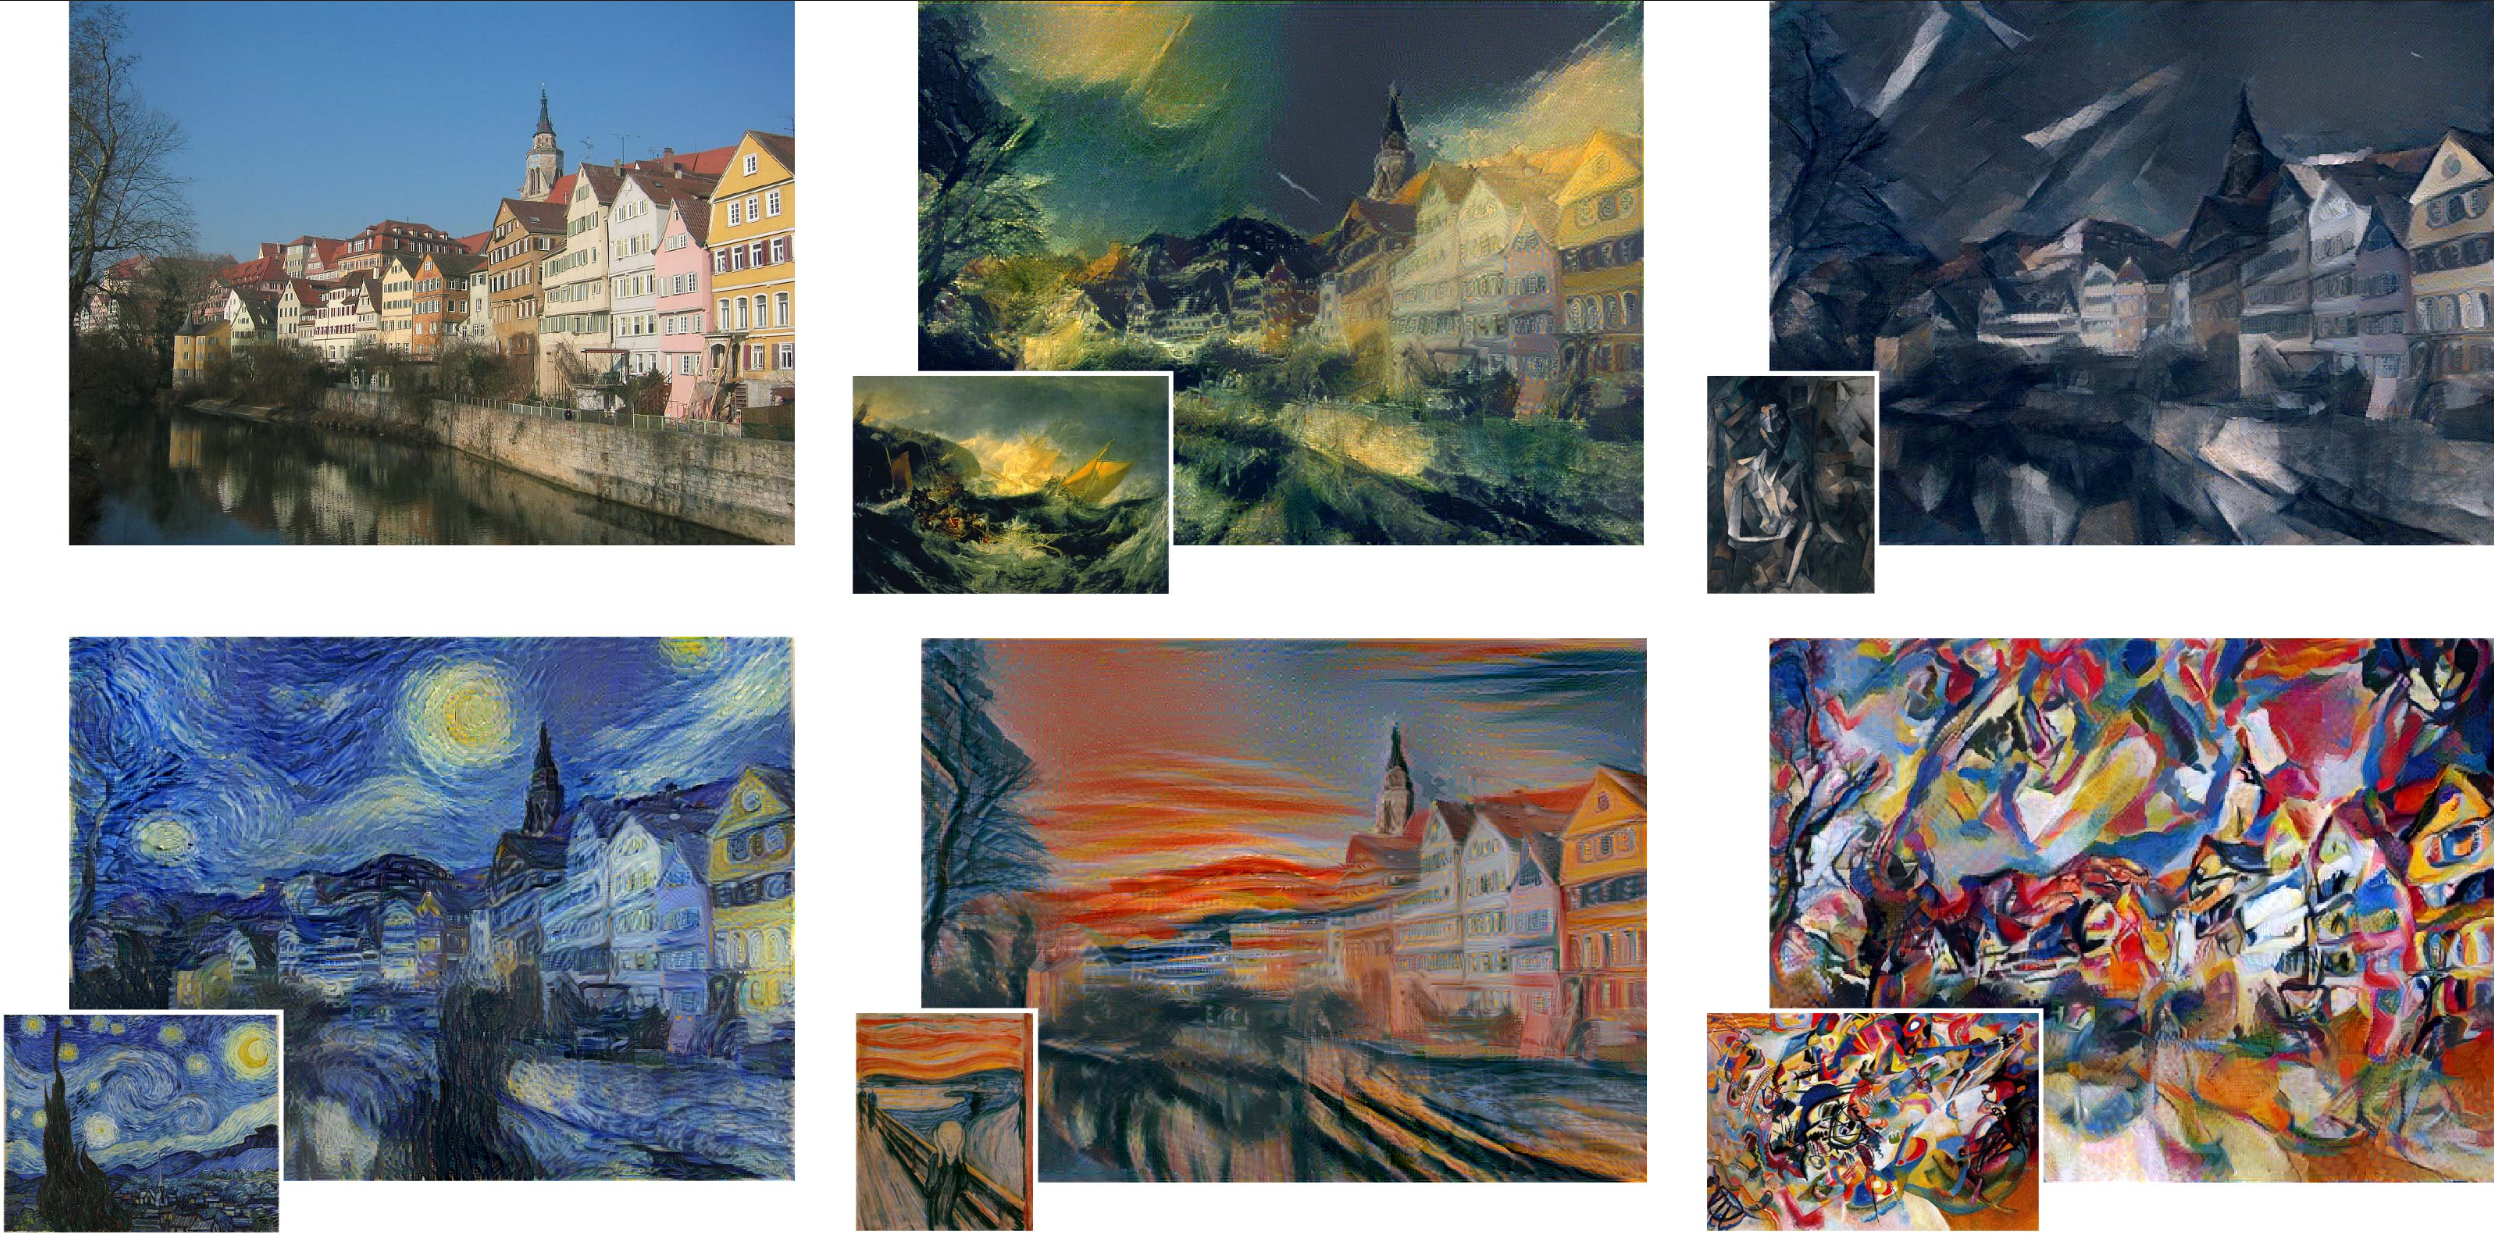
\includegraphics[width=\linewidth]{resources/styleg.png}
 \captionof{figure}{Style transfer examples}
 \label{fig:style_ex}
\end{Figure}

\section{Generative Adversarial Networks}
Goodfellow's approach was to use two models to solve the problem. The "generator" network generates candidates in the form of randomly sampled noise from true data distribution, while the "discriminator" network evaluates these samples. These two networks play a min-max game where the generator tries to generate "fake" samples that it thinks the discriminator will think are real, and "real" samples that it thinks the discriminator will think are fake, while the discriminator tries to "beat" the generator network by correctly classifying the incoming samples.
Over the years after Goodfellow's original GAN paper, the performance of these networks has improved quite a bit. Alec Radford's DCGANs\cite{radford_metz_chintala_2015} proposed the use of convolutional networks in place of fully connected networks, which improved the results and performance of the models. Further improvements for implementing GANs on large scale images such as Andrew Brock's 2018 \cite{DBLP:journals/corr/abs-1809-11096} paper on the subject, further proved that GANs could be used for larger resolution images.

\section{StyleGAN}

Tero Karras from NVIDIA proposed in 2018 an alternative GAN architecture to implement a style-transfer network.\cite{DBLP:journals/corr/abs-1912-04958} 

While the latent space code is provided to the generator network through it's input layer, Karras chooses to omit the input layer altogether and start from a pre-learned constant. 

NVIDIA's team provides their novel generator with a direct means to generate stochastic detail by using explicit noise inputs, as single-channel images consisting of uncorrelated Gaussian noise. These noise images are broadcasted to all feature maps using the learned per feature scaling factors and then added again to the output of their respective convolutions. 

Karras et al. had amazing results using this approach, as seen in Figure \ref{fig:style_face}.

\begin{Figure}
 \centering
 \includegraphics[width=8cm]{resources/styleface.png}
 \captionof{figure}{StyleGAN results}
 \label{fig:style_face}
\end{Figure}

In 2019, NVIDIA's team set out to improve StyleGAN by targeting several of it's characteristic artifacts\cite{DBLP:journals/corr/abs-1912-04958}. In this paper, the team sets out to redesign the generator normalization and regularize the generator to encourage good conditioning in the mapping from latent codes to images. 

To remove normalization artifacts, NVIDIA's team identifies an AdaIN operation that normalizes mean and variance of every feature map sepearately, destroying any information found in the magnitudes of the features relative to each other. They instead remove the normalization step from the generator, causing the droplet artifacts to dissapear.

On the other hand, the generator's architecture is revisited completely. Where the original StyleGAN applies bias and noise within the style block, more predictable results are obtained by their modification, which is moving these operations outside of the style block, operating on normalized data. They also remove the application of bias, noise and normalization to the constant input without any observable drawback in performance or quality.

\subsection{StyleGAN2}
Later in 2020, Karras' team releases the "StyleGAN2" paper \cite{DBLP:journals/corr/abs-2006-06676}. This time around, Karras and his team set out to improve their StyleGAN to work with limited amounts of data. They propose the implementation of an adaptive discriminator augmentation mechanism that stabilizes training when the dataset used is small. They demonstrate that results are not greatly affected even without modifying the loss functions or the architecture of the network.

We tried implementing a variant of the StyleGAN2 for use in our project initially, but our results proved to be too slow, and too poor compared to Karras' team's release. 

\section{Method}

In this section, we will describe the used dataset for emotion recognition and style transfer, and the methods used for face recognition. We also propose the methods we think are needed in order to achieve a minimum viable product for our robot.


To achieve a MVP (Minimum Viable Product), and be worthy of a MSc project, we set our goals as the following:
\begin{itemize}
  \item Remove the need to use Google's Cloud API for all computer vision tasks, implementing local solutions.
  \item Implement new routines involving engaging computer vision algorithms like Style Transfer.
  \item Make the robot completely autonomous: no need for an outlet or a server to offload the heavy algorithm computations.
  \item Achieve a real-time representation of the robot's image processing.
  \item The user should easily be able to obtain the style transferred files.
  \item The visual representation on the screen should be at least visually pleasing enough that users will want to keep it on as a background element.
\end{itemize}

\subsection{Face detection and emotion recognition}

Previously, our pipeline for the robot required sending images to Google's Cloud Services (GCS) for emotion recognition. As we have removed GCS, this is no longer the case. To replace the previous face detection + emotion detection parts of the pipeline, we need to implement local methods face detection and emotion detection based off state of the art methods. 

Face detection serves two purposes for our robot: the first is allowing the arm to follow a subject should it approach the limits of the camera's viewing angle. It also serves to improve emotion detection, as described in Gunwan et al.\cite{haarcrop}, a neural network trained on cropped faces performs optimally on similiarly cropped images. We propose using a Haar-Cascade classifier to detect faces.

Emotion detection will be used to change the context of the style transfer network, loosely adapting the target style transfer to a user's visible emotional status

\begin{figure}
  \centering
  \includegraphics[width=\textwidth]{resources/state_machine.png}
  \caption{Robot flow diagram.}\label{fig:state_machine}
\end{figure}



\hl{TODO}



For our face detection, we have to consider that our robotic arm does not move smoothly, and covers a big arc of movement on every sweep. To counter this, we propose optical flow detection to stabilize frames with a high likelyhood of having a face in them, and only run our face and emotion detection algorithm on those frames, reducing the performance impact of these algorithms.

On our previous implementation, we could detect faces at a rate of 1 face detection per 3 seconds given the overhead the program needed to make all the necessary preparations for the GCS-based emotion detection. 

As we are already producing optical flow calculations, we can use a "bundle" of similiarly-flowing pixels to detect wether a person has left the frame, and use face detections more sparingly as it would not be necessary.

The arm aims to keep the people in the frame within the middle third of the frame as long as it's movement allows it. If there is more than one person in frame, we keep track of the position of the face belonging to the last person that entered the frame, and use that detection for the centering algorithm. The algorithm is able to keep track of multiple faces in the frame, but we found that movement would be extremely jerky when we tried to keep the camera centered in the middle of the faces, and the field of view is wide enough for this to be unnecessary. 

\hl{TODO}


At this point in the timeline, each frame takes \hl{[TIME]} seconds to process and be prepared for the next part of the pipeline. This already represents a \hl{TIMES}X speedup compared to the processing time required per frame on the previous implementation, and it is done completely locally.


\hl{TODO}


This train of thought proved to be flawed, as we minimally improved the speed of inference of the models, while taking a massive hit on image quality for style transfer.

\hl{TODO}


\section{Experiments}

\begin{itemize}
  \item Fast neural Style: pytorch vgg19 experiments.
  \item Emotion detection: FER
  \item 
\end{itemize}


\section{Results}
\begin{itemize}
  \item Face detection performance (time per frame)
  \item Emotion detection performance (time per frame)
  \item style change on the fly performance (time per frame)
  \item generate high resolution style transfer + save+send image performance (seconds)
\end{itemize}

\subsection{Preprocessing: face and emotion detection}

We measure the performance of our face and emotion detection algorithms by how much time it takes for them to produce a result, as each passing frame affects the quality of the final product. 

Towards real-time: detecting face->crop->emotion detector if face is persistent 

-> switch style context if
  emotion is persistent.
Explanation about the performance evaluation procedure and results analysis.

\begin{figure}[t]
  \centering
     \begin{subfigure}{0.49\linewidth} \centering
       \includegraphics[scale=0.49]{resources/emotionvsframe.png}
       \caption{Emotion variation by frame of a sample.}\label{fig:figA}
     \end{subfigure}
     \begin{subfigure}{0.49\linewidth} \centering
       \includegraphics[scale=0.49]{resources/timeseriesplot.png}
       \caption{Time needed to process a frame.}\label{fig:figB}
     \end{subfigure}
  \caption{Overall caption} \label{fig:emotionandtime}
  \end{figure}


\subsection{Style transfer}

We started by taking Karras' team StyleGAN2 implementation and trying to tweak it to run on the Raspberry Pi 4s hardware. 


The purpose of using Karras' model was to try to minimize the requirements for inference of a trained model following their architecture. Our logic was that minimizing the footprint of the model, inference would be fast enough to complete in real time for our robot. To achieve this, we reduced the dimensions of several layers of the model to output images at a 128x128 pixel resoluion, with the intent of upscaling the images ran taken through the inference in real-time to achieve a good framerate, and switch to a larger model when saving an image for the user. 

\section{Conclusions}

Summary about the degree of achievement according to the given problem and the adopted hypothesis; and outline about open research lines...


\appendices
\section{Appendix title}
Appendix one text goes here.


% use section* for acknowledgement
\section*{Acknowledgment}


The authors would like to thank...


% Can use something like this to put references on a page
% by themselves when using endfloat and the captionsoff option.
\ifCLASSOPTIONcaptionsoff
  \newpage
\fi



% trigger a \newpage just before the given reference
% number - used to balance the columns on the last page
% adjust value as needed - may need to be readjusted if
% the document is modified later
%\IEEEtriggeratref{8}
% The "triggered" command can be changed if desired:
%\IEEEtriggercmd{\enlargethispage{-5in}}

% references section

% can use a bibliography generated by BibTeX as a .bbl file
% BibTeX documentation can be easily obtained at:
% http://www.ctan.org/tex-archive/biblio/bibtex/contrib/doc/
% The IEEEtran BibTeX style support page is at:
% http://www.michaelshell.org/tex/ieeetran/bibtex/
%\bibliographystyle{IEEEtran}
% argument is your BibTeX string definitions and bibliography database(s)
%\bibliography{IEEEabrv,../bib/paper}
%
% <OR> manually copy in the resultant .bbl file
% set second argument of \begin to the number of references
% (used to reserve space for the reference number labels box)

\medskip

\bibliographystyle{IEEEtran}
\bibliography{references.bib}


% biography section
% 
% If you have an EPS/PDF photo (graphicx package needed) extra braces are
% needed around the contents of the optional argument to biography to prevent
% the LaTeX parser from getting confused when it sees the complicated
% \includegraphics command within an optional argument. (You could create
% your own custom macro containing the \includegraphics command to make things
% simpler here.)
%\begin{IEEEbiography}
%    [{\includegraphics[width=1in,height=1.25in,clip,keepaspectratio]{mshell}}]{Michael Shell}
% or if you just want to reserve a space for a photo:

% You can push biographies down or up by placing
% a \vfill before or after them. The appropriate
% use of \vfill depends on what kind of text is
% on the last page and whether or not the columns
% are being equalized.

%\vfill

% Can be used to pull up biographies so that the bottom of the last one
% is flush with the other column.
%\enlargethispage{-5in}



% that's all folks
\end{document}


